\begin{frame}{Area Under Curve}
\begin{center}
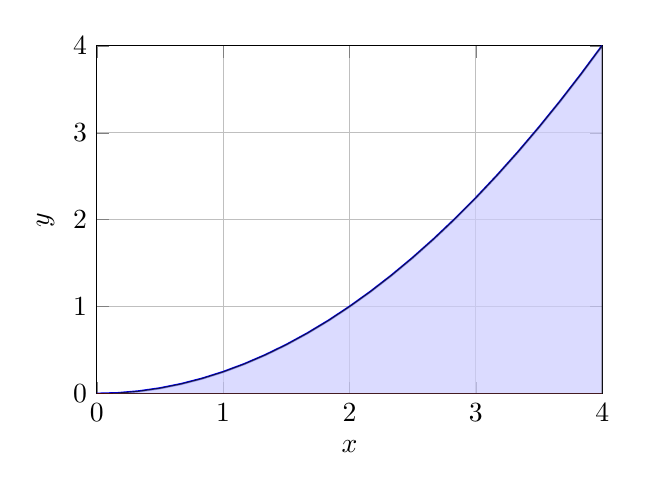
\begin{tikzpicture}
\begin{axis}[
    xlabel={$x$},
    ylabel={$y$},
    grid=both,
    xmin=0, xmax=4,
    ymin=0, ymax=4,
    width=8cm,
    height=6cm
]
\addplot[thick, blue, domain=0:4] {x^2/4};
\addplot[thick, red, domain=0:4] {0};
\addplot[fill=blue!20, opacity=0.7, domain=0:4] {x^2/4} \closedcycle;
\end{axis}
\end{tikzpicture}
\end{center}

\footnotesize
\texttt{\textbackslash addplot[fill=blue!20, opacity=0.7] fill between[of=A and B];}
\end{frame}